\newpage
\clearpage

\section{Redes Neurais Profundas}
\label{deep:deep}
Inspiradas no modelo de sistema nervoso de seres inteligentes, as redes neurais são compostas por um conjunto interconectado de neurônios de modo que, assim como o sistema humano, um neurônio, quando conectado com outros neurônios, pode comunicar impulsos nervosos por meio de sinapses. A representação do modelo humano pode ser observado na Figura \ref{deep:fig:1}.

\begin{figure}[H]
    \centering
    \caption{Representação do neurônio biológico.}
    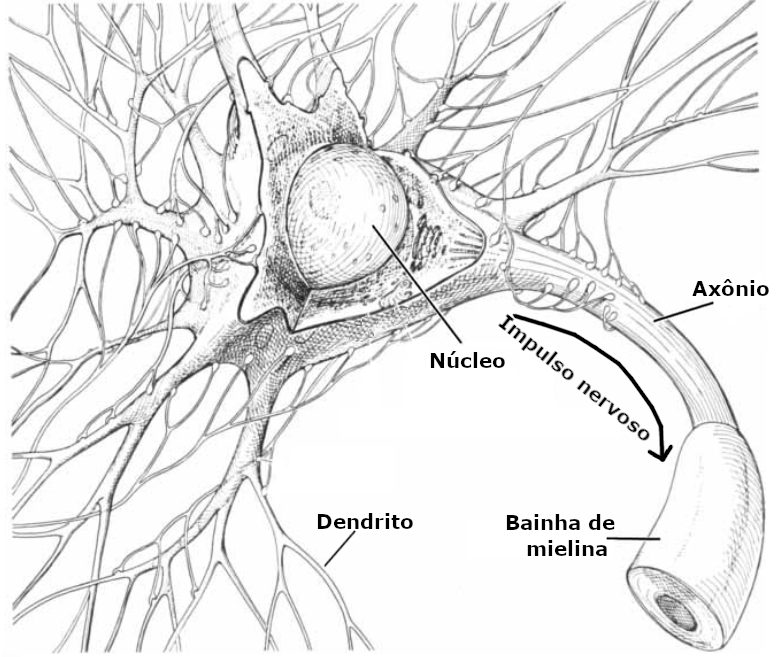
\includegraphics[width=1\linewidth]{recursos/imagens/deep/neuronio.png}
    \label{deep:fig:1}

    Fonte: traduzido e adaptado de \cite{Stevens1979}.
\end{figure}

Dentre as representações matemáticas, destaca-se o modelo pioneiro desenvolvido por \cite{mcculloch1943logical}, que baseado no neurônio biológico busca definir uma saída binária, a partir de entradas que são recebidas por meio dos dendritos, sendo assim, sua representação matemática se dá pela equação:

\begin{equation}
    \label{deep:eq:1}
    J = \sum_{i = 1}^{n} x_i.
\end{equation}

Para a Equação \ref{deep:eq:1} e para a Figura \ref{deep:fig:2}, é importante dizer que $J$ representa a saída do neurônio, enquanto $x_i$ é a entrada a partir de $i$. Logo, é possível observar que por meio dos dendritos ocorre a entrada dos dados que é somada (ponderadamente) no núcleo $\sum_{i = 1}^{n} x_i$. Por fim, vale citar que $(x_1, ..., x_n)$ é assimilado aos dendritos e, além disso, é comum ver a representação do modelo supracitado através da seguinte imagem (Figura \ref{deep:fig:2}):

\begin{figure}[H]
    \centering
    \caption{Representação matemática de neurônio \cite{mcculloch1943logical}.}
    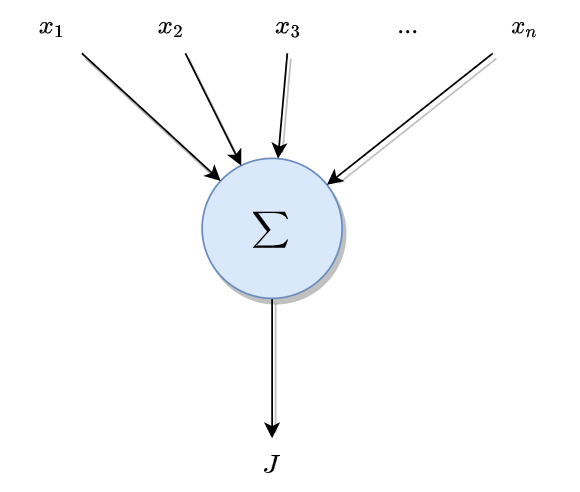
\includegraphics[width=1\linewidth]{recursos/imagens/deep/neuronio_mc.png}
    \label{deep:fig:2}

    Fonte: do próprio autor. Inspirado em \cite{mcculloch1943logical}.
\end{figure}

A partir do modelo de neurônio desenvolvido por \cite{mcculloch1943logical},  outros trabalhos foram desenvolvidos, no qual vale ressaltar o trabalho de \cite{Rosenblatt1958}, que propôs um modelo de neurônio e o nomeou de Perceptron, o qual tem como princípio o uso de uma saída binária. Logo, destaca-se que a sua função de ativação é dada de forma condicional e pode ser representada pela Equação \ref{deep:eq:2} \citep{Rosenblatt1958}.

\begin{equation}
    \label{deep:eq:2}
    A(Y') = \left\{\begin{matrix}
     1,& se \sum_{N}^{i=1} w_i x_i + b \geq 0 \\ 
     0,& caso \;  contrario.
    \end{matrix}\right.
\end{equation}

Dessa forma, entende-se que $b$ representa o viés que determina um limiar para a ativação do neurônio. O vetor $\textbf{x}$, corresponde à entrada da rede, enquanto $\textbf{W}$ é a matriz de pesos que deve ser inicializada aleatoriamente e é ajustada no decorrer do treinamento.

Dentre as vantagens para o modelo Perceptron, pode-se salientar a sua aptidão para resolução de problemas lógicos, como também para problemas linearmente separáveis, todavia, em meio às suas limitações, reforça-se sua imperícia em relação a problemas não linearmente separáveis como os do exemplo na Figura \ref{deep:fig:3}\subref{deep:fig:3.2}.

\begin{figure}[H]
   \caption{Representação de problemas linearmente e não linearmente separáveis.}
   \centering
   \label{deep:fig:3}
    \begin{subfigure}[t]{0.45\textwidth}
        \centering
        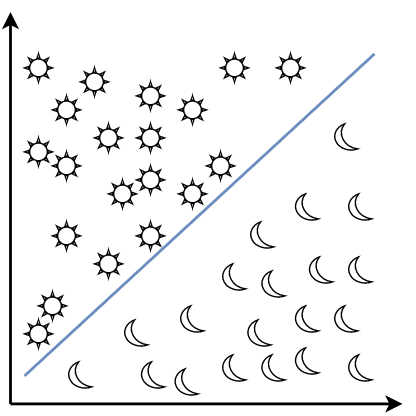
\includegraphics[height=1.5in]{recursos/imagens/deep/l_separavel.png}
        \caption{Problema linearmente separável.}
        \label{deep:fig:3.1}
    \end{subfigure}%
    ~ 
    \begin{subfigure}[t]{0.45\textwidth}
        \centering
        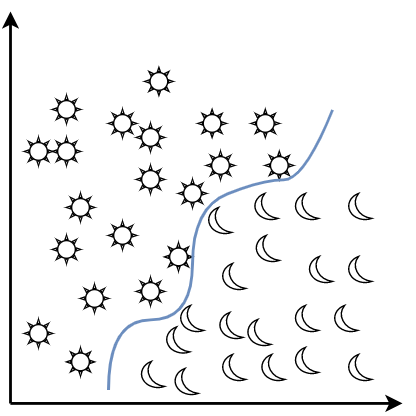
\includegraphics[height=1.5in]{recursos/imagens/deep/nl_separavel.png}
        \caption{Problema não linearmente separável.}
        \label{deep:fig:3.2}
    \end{subfigure}%

    Fonte: do próprio autor.
\end{figure}

Para suprir essa necessidade de trabalhar com problemas não lineares, \cite{Werbos:74} realizou uma proposta de utilizar várias camadas de neurônios Perceptron juntos, de modo que obrigatoriamente possuísse uma camada de entrada, oculta e de saída. Assim, esse modelo - nomeado de \textit{Multi Layer Perceptron} (MLP) \citep{Werbos:74} e representado na Figura \ref{deep:fig:4} - possibilitou o trabalho com funções de ativação não lineares e o desenvolvimento de técnicas de aprendizado, como a \textit{backpropagation}, desenvolvida por \cite{rumelhart1986learning}, a qual será detalhada na Seção \ref{deep:backprop}.

\begin{figure}[H]
    \centering
    \caption{Representação do modelo MLP.}
    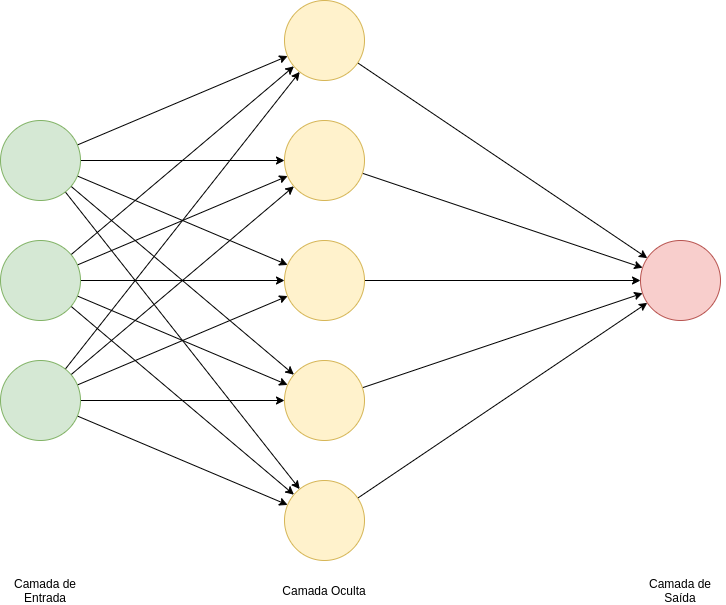
\includegraphics[width=1\linewidth]{recursos/imagens/deep/mlp.png}
    \label{deep:fig:4}

    Fonte: do próprio autor.
\end{figure}

Entretanto, com o uso dos modelos citados, a tentativa de resolver problemas de nível de complexidade maior e o desenvolvimento de trabalhos que contribuíssem para o estado-da-arte, percebeu-se que ao adicionar mais camadas era possível trabalhar com uma base de dados maior e mais complexa, além de obter melhores resultados e uma etapa maior de treinamento, o que deu origem às intituladas redes neurais de aprendizado profundo, ou em inglês, \textit{deep learning} \citep{Goodfellow2016}. No que lhe concerne, essas possuem o princípio de aprender os parâmetros e representações dos dados de acordo com as suas interações \citep{ponti2018funciona}, assim, possibilitando o algoritmo combinar parâmetros e simplificá-los antes de propagar a representações que consideram as demais camadas \citep{Goodfellow2016}.

Além disso, vale citar que um diferencial dos modelos de \textit{deep learning} se materializa no fato de que seus neurônios tornam-se especialistas em determinados objetivos e tornam-se diferentes um dos outros, como o que ocorre com as CNNs que têm neurônios responsáveis por extrair características, enquanto os neurônios da camada final fazem classificação (ou regressão), simulando o tráfego da informação no córtex visual humano.

Destarte, o uso e desenvolvimento de \textit{deep learning} tem se popularizado e sido considerado a resposta para problemas de diversas áreas, como segmentações em vários contextos, desenvolvimentos de carros autônomos, segurança, otimização de modelos de busca e afins \citep{Ghosh2019}, sendo que essa popularização é propicia devido: 1) ao desenvolvimento acelerado de \textit{hardwares} que acrescentam velocidade no treinamento dessas redes e 2) ao grande aumento de dados variados (com adventos como o \textit{big data}) \citep{Szegedy2015, ponti2018funciona}.

Por conseguinte, nas demais seções deste capítulo serão apresentadas algumas variações de funções de ativação (Seção \ref{deep:activation}), sobre o processo de treinamento (Seção \ref{deep:train}) e de testes (Seção \ref{deep:test}) e, finalmente, sobre redes neurais convolucionais (Seção \ref{deep:CNN}).


\subsection{Funções de Ativação}
\label{deep:activation}

Quanto às funções de ativação, destaca-se que na seção anterior foi apresentada uma função de ativação binária, todavia, existem outras funções de ativação que foram estudadas e são utilizadas para uma melhor adequação em contextos específicos.

A função de ativação, como citado brevemente a priori, é calculada pelo neurônio e disseminada para os próximos neurônios.  Para essa Seção o valor calculado $\sum_{i = 1}^{N} w_ix_i +b$ (entrada da função de ativação) será representado por $Y'$, de modo que poderemos ver sua atuação, a seguir, nas funções de ativação Limiar, Linear, Sigmóide, ReLU e Sofmax.


\subsubsection{Função Limiar}
A função limiar define um limite (\textit{threshold}) $\gamma$, em que valores abaixo de $\gamma$ indicam uma saída sem excitação, para valores acima de $\gamma$, há a excitação para o neurônio, utilizando assim, de medidas binárias, que normalmente são representadas por 0 e 1, respectivamente.

Essa função se faz eficiente quando trabalhando com 2 classes, todavia passa a ter dificuldades quando atuando em problemas multi-classes, visto que não garante a excitação de um único neurônio da camada de saída.

Em relação à função de ativação ($f(Y')$) desenvolvida e utilizada no Perceptron, pode-se dizer que o valor de $\gamma = 0$, é definida matematicamente por \cite{mcculloch1943logical} segundo a Equação \ref{deep:eq:3}:

\begin{equation}
    \label{deep:eq:3}
    f(Y') = \left\{\begin{matrix}
     1,& se \; Y' \geq \gamma \\ 
     0,& \text{caso contrário}.
    \end{matrix}\right.
\end{equation}


\subsubsection{Função Linear}
Para suprir a problemática de trabalhar com contextos de multi-classe, saídas contínuas podem ajudar quanto à interpretação e subjugar o problema da função limiar, sendo que para essa atividade é adequado o uso da função linear. Porém, é importante ter conhecimento que os resultados expressos por funções lineares também são lineares, não sendo recomendado o seu uso para atividades que não pertencem a problemas lineares. A função linear pode ser expressa pela Equação \ref{deep:eq:5}, segundo \cite{Rosenblatt1958}:

\begin{equation}
    \label{deep:eq:5}
    f(Y') = \alpha Y'.
\end{equation}


\subsubsection{Função Sigmoide}
As funções sigmoides não se limitam a problemas lineares, assim sendo caracterizada como função de ativação não-linear e possibilitando o uso de probabilidade quanto à saída do neurônio.

Essa função de ativação também é cognominada e expressa por \cite{glorot2011deep} como função logística. Sua expressão matemática se dá por:

\begin{equation}
    \label{deep:eq:6}
    f(Y') = \frac{1}{1 + e^{Y'}}.
\end{equation}

A desvantagem dessa função encontra-se em situações de variação do eixo x, em que há uma  dissipação do seu gradiente, implicando em um aprendizado mais lento nos neurônios das primeiras camadas em relação aos das últimas, tendo em vista os valores muito pequenos no início.

\subsubsection{Função ReLU}
A função desenvolvida por \cite{Hahnioser2000} e popularmente conhecida como ReLU (\textit{Rectified Linear Unit}) se faz útil nas camadas ocultas da rede neural \citep{Goodfellow2016}, sendo que sua utilidade é destacada por não permitir resultados negativos \citep{Dahl2013} e ter uma rápida convergência, principalmente quando comparada à função sigmoide, além de não passar por problemas de perda do gradiente. Sua função é definida pela Equação \ref{deep:eq:7} \citep{Hahnioser2000}:

\begin{equation}
    \label{deep:eq:7}
    f(Y') = \max(0,Y').
\end{equation}

\subsubsection{Função Softmax}
\label{deep:soft}
Por fim, quando se trata da função Softmax, dois processos são essenciais para a convergência do modelo em questão, sendo ele: 1) realizar a exponenciação dos valores de cada neurônio e 2) realizar a normalização de cada valor pela soma de todos os valores exponenciado no passo anterior, assim, definido uma saída no domínio $[0,1]$, fazendo com que a soma total seja sempre 1 \citep{kotu2018data} e que a saída da função seja a distribuição de probabilidade da classe. Esse comportamento garante que a função Softmax seja recomendada para problemas de multi-classe, além de determinar as probabilidades de cada uma das classes.

Entretanto, em um problema de k-classes, a função Softmax pode ser expressa pela Equação \ref{deep:eq:8} \citep{kotu2018data}:

\begin{equation}
    \label{deep:eq:8}
    f(Y = \boldsymbol{k}) = \frac{e^{z_k}}{\sum_{i=1}^{\boldsymbol{k}} e^{Y'}},
\end{equation}
tendo $z_k$ como cada entrada do vetor $\boldsymbol{k}$.


\subsection{Treinamento}
\label{deep:train}

Definida como uma fase crucial por \cite{ponti2018funciona}, a fase de treinamento está relacionada com a minimização da função de custo (que será abordada na Seção \ref{deep:cust}), de modo que a rede ajuste os seus parâmetros iterativamente. Essas interações são explicadas por cada laço de repetição que ocorre com cada exemplo, sendo esperado que o erro propagado na rede seja minimizado. Assim, quando as interações ocorrem por todo o conjunto de dados de treinamento, é dito que aconteceu a ocorrência de uma época.

Normalmente, os passos realizados em uma época são os seguintes: 1) iniciação; 2) escolha de uma amostra (normalmente de modo aleatório); 3) cálculo de saída através de função de ativação, além do, 4) erro através de função de custo e \textit{backpropagation}; 5) modificação dos pesos de cada camada da rede e; 6) uma nova interação, até que tenha se passado por todas as instâncias do conjunto de treinamento.

Além da seleção aleatória, vale citar que normalmente os pesos são iniciados de modo aleatório nas camadas, assim como os hiperparâmetros, que são definidos pelo usuário na etapa de inicialização, por exemplo, o valor da taxa de aprendizado.

Nesta seção, será brevemente discorrido sobre as funções de custo (Seção \ref{deep:cust}), que indicam o erro da rede em relação ao conjunto de treinamento, sobre as funções de otimização (Seção \ref{deep:optimization}), que auxiliam na convergência do modelo e, por fim, sobre o algoritmo \textit{backpropagation} (Seção \ref{deep:backprop}), que propaga o erro para as camadas internas da rede.


\subsubsection{Função de Custo}
\label{deep:cust}

As funções de custo, (do inglês, \textit{loss functions}) são responsáveis por realizar a avaliação do modelo durante a fase de treinamento, de certa maneira, avaliando quão perto o aprendizado do modelo está da resposta correta.

Em meio às avaliações utilizadas como métrica para o cálculo da função de custo em relação a problemas como o de regressão, destaca-se o erro quadrático médio (ou \textit{Mean Squared Error}, MSE)\citep{Wang2004}, em que para o âmbito de visão computacional e trabalho com imagens, comumente ocorre da saída da rede neural ser uma imagem, a partir de onde calcula-se o MSE dos pixeis existentes entre a imagem predita $\boldsymbol{y'}$ e a imagem original $\boldsymbol{y}$. Assim, supondo que M e N sejam as dimensões da imagem, o MSE é calculado pela equação:

\begin{equation}
    \label{deep:eq:9}
    MSE(\boldsymbol{y}, \boldsymbol{y'}) = \frac{1}{MN} \sum_{i=1}^{M} \sum_{j=1}^{N} (\boldsymbol{y}_{i,j} - \boldsymbol{y'}_{i,j})^2.
\end{equation}

Ainda quanto as métricas para a realização de avaliação em relação a imagens, existem várias delas descritas na literatura, todavia,  cada uma delas possui seu uso especificado para o problema que deseja resolver, por exemplo o caso das métricas para segmentações panópticas na Seção \ref{semantic:metrics}.


\subsubsection{Função de Otimização}
\label{deep:optimization}

O grande objetivo das funções de otimização no contexto de \textit{deep learning}, de certa forma, podem ser resumidos pela Equação \ref{deep:eq:10} e visualizada na Figura \ref{deep:fig:otimizacao}, em que almeja-se uma minimização global da função de custo $f(\boldsymbol{x})$ através de pesos $\boldsymbol{\theta}$ e de entradas $\boldsymbol{x}$:

\begin{equation}
    \label{deep:eq:10}
    \boldsymbol{\theta}* = argmin(f(\boldsymbol{x};\boldsymbol{\theta})).
\end{equation}

\begin{figure}[H]
    \centering
    \caption{Representação da otimização da função de custo em um espaço de características.}
    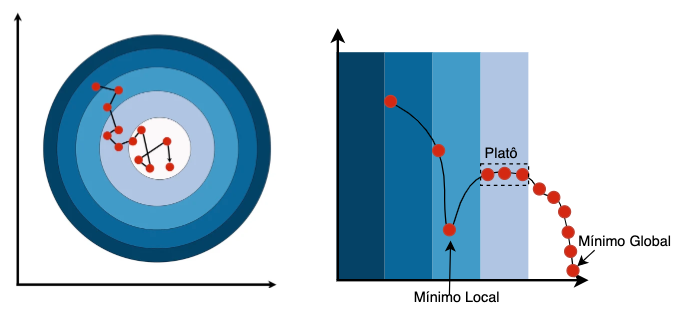
\includegraphics[width=1\linewidth]{recursos/imagens/deep/funcao_otimizacao.png}
    \label{deep:fig:otimizacao}

    Fonte: do próprio autor. Inspirado em \cite{MontesinosLopez2022ArtificialOutcomes} e \cite{Geron2017Hands-onSystems}.
\end{figure}

A Figura \ref{deep:fig:otimizacao} proporciona uma visualização de alguns desafios para as funções de otimização, sendo 1) mínimos locais e 2) platô (\textit{plateau}, em inglês). Um mínimo local representa um ponto que é o menor em comparação com outros pontos em sua vizinhança próxima. Entretanto, é importante notar que um mínimo local nem sempre corresponde ao menor valor em todo o espaço de características. Dessa forma, a função de custo pode apresentar vários mínimos locais, o que frequentemente dificulta a busca pelo mínimo global desejado na otimização\citep{Goodfellow2016}. Já os pontos de platô indicam áreas onde o valor da função de custo permanece estagnado. Nestes locais, os gradientes são muito semelhantes, o que torna desafiadora a otimização do modelo \cite{Goodfellow2016}.

Em meio às diversas funções disponíveis, considera-se que o método mais utilizado é o de gradiente descendente estocástico, ou em inglês, \textit{stochastic gradient descendent} (SGD) desenvolvido inicialmente por \cite{cauchy1847methode}, assim como suas variações \citep{Goodfellow2016}, sendo que o gradiente descendente estocástico é considerado como uma adaptação do gradiente descendente e que causa a aceleração do treinamento na maioria das vezes por selecionar aleatoriamente apenas uma parcela do conjunto de treinamento. Todavia, segundo \cite{Goodfellow2016}, há casos em que o SGD não tem bom desempenho para convergir e por conta disso são estudadas suas variações.

De qualquer modo é interessante ter consciência que até então não há um consenso na escolha do melhor método de otimização para problemas em gerais, segundo aborda \cite{Goodfellow2016}.


\paragraph{Gradiente Descendente}
\label{deep:optimization:graddesc}
O método do gradiente descendente representa uma técnica de otimização com a capacidade de encontrar soluções ideais em uma variedade de contextos, operando de maneira iterativa \citep{Geron2017Hands-onSystems}. Seu processo, por sua vez inicia-se com o calculo dos gradientes locais resultados da função de custo $f(\boldsymbol{\theta})$ bem como com a atualização do o valor dos pesos $\boldsymbol{\theta}$ com base na magnitude do gradiente e na direção indicada pelo calculo das derivadas. A derivada da função $f'(\boldsymbol{\theta})$, determina a inclinação da função $f(\boldsymbol{\theta})$ no ponto $\boldsymbol{\theta}$, permitindo a analise de como a variação nos valores de entrada $\boldsymbol{x}$ da função se reflete em mudanças correspondentes nos valores de saída \citep{Goodfellow2016}, sendo possível minimizar a função movendo os valores de $\boldsymbol{\theta}$ em pequenos incrementos no sentido oposto ao da derivada.

Em situações envolvendo funções com múltiplas variáveis de entrada, as derivadas parciais $\frac{\partial}{\partial_{\theta_{i}}}f(\boldsymbol{\theta})$ são levadas em consideração para mensurar o quanto a função $f$ varia quando a entrada $x_i$ é alterada no ponto $\boldsymbol{\theta}$, assim o gradiente passa a ser representado por um vetor que encapsula os valores de todas as derivadas parciais \citep{Goodfellow2016}, sendo expresso por: $\nabla_{\boldsymbol{\theta}} f(\boldsymbol{\theta})$.  Por fim, a atualização dos parâmetros ocorre conforme a Equação \ref{deep:eq:graddesc} descrita por \cite{Goodfellow2016}:

\begin{equation}
    \label{deep:eq:graddesc}
    \boldsymbol{\theta}' = \boldsymbol{\theta} - \epsilon \nabla_{\boldsymbol{}{\theta}} j(\boldsymbol{}{\theta}).
\end{equation}

Dessa forma, o valor de entrada $\boldsymbol{x}$ é ajustado por meio da multiplicação das derivadas parciais pela taxa de aprendizado $\epsilon$ que pode ser vista na Figura \ref{deep:fig:otimizacao} com os círculos vermelhos.

\paragraph{Gradiente Descendente Estocástico}
\label{deep:optimization:sgd}
O SGD é amplamente adotado devido à sua eficiência em modelos de aprendizado profundo e conjuntos de dados em larga escala \citep{Goodfellow2016}. No entanto, é importante mencionar suas limitações. O SGD não assegura a convergência e é sensível aos valores iniciais do modelo. No entanto, essas desvantagens não excluem sua utilidade, especialmente quando combinado com técnicas como normalização e o uso de \textit{momentum} \cite{Goodfellow2016}.

A fórmula do SGD emprega a derivada da função $f(\boldsymbol{x})$ em relação a $\boldsymbol{y} = f(\boldsymbol{x})$. Essa modificação de $\boldsymbol{x}$, impulsionada pela derivada, resulta em melhorias em $\boldsymbol{y}$. A representação do SGD é apresentada na Equação \ref{deep:eq:sgd}, proposta por \cite{Goodfellow2016}:

\begin{equation}
\label{deep:eq:sgd}
g = \nabla_{\boldsymbol{\theta}} \left(\frac{1}{m} \sum\limits_{i=1}^{m}L(f(\boldsymbol{x}^{(i)}; \boldsymbol{\theta}), \mathbf{y}^{(i)})\right),
\end{equation}
onde $L(x,y)$ é a função de custo, $\boldsymbol{x}$ representa a entrada, $\boldsymbol{y}$ indica a saída esperada, $m$ é o número de exemplos no conjunto de dados, e $f(\boldsymbol{x}^{(i)}; \boldsymbol{\theta})$ é a saída da rede para o enésimo exemplo $\boldsymbol{x}^{(i)}$ com o conjunto de pesos $\boldsymbol{\theta}$.

\paragraph{Adam}

\paragraph{Taxa de Aprendizado Dinâmica}

\paragraph{Parada antecipada}
\label{deep:optimization:early_stoping}

Ao configurar os hiperparâmetros de um modelo, é crucial considerar a quantidade de épocas pelas quais o conjunto de dados deve passar durante o treinamento. Essa escolha tem um impacto significativo nos fenômenos discutidos na Seção \ref{deep:overunder}. Optar por um número insuficiente de épocas frequentemente resulta em \textit{underfitting}, enquanto um número excessivo pode levar ao \textit{overfitting}. Surge, então, a pergunta fundamental: \quotes{Qual é o número ideal de épocas para cada problema?}

Para abordar essa questão, diversos estudos têm sido realizados com o intuito de encontrar critérios de parada no treinamento que minimizem ou previnam esses problemas \citep{Prechelt1998AutomaticCriteria}. Além disso, pesquisas recentes tentam antecipar situações de \textit{overfitting} e \textit{underfitting}, interrompendo o treinamento antes que afete o desempenho do modelo \citep{VilaresFerro2023EarlyNetworks}. Existem múltiplos métodos disponíveis para essa tarefa, sendo a parada antecipada (do inglês, \textit{early stopping}) um dos mais populares, podendo ser considerado uma forma de regularização, tal como o decaimento de pesos \cite{VilaresFerro2023EarlyNetworks}.

A aplicação da Parada Antecipada implica calcular a precisão da classificação nos dados de validação ao final de cada época \citep{Prechelt1998AutomaticCriteria}. Quando a precisão para de melhorar, encerramos o treinamento. Isso simplifica a definição do número de épocas, pois não é necessário explicitamente determinar como ele depende de outros hiperparâmetros - essa adaptação é feita automaticamente. Ademais, a Parada Antecipada atua como um mecanismo automático de prevenção ao \textit{overfitting}. Embora, em estágios iniciais de experimentação, possa ser útil desativar temporariamente a Parada Antecipada para identificar sinais de \textit{overfitting} e, assim, ajustar a abordagem de regularização.

A implementação efetiva da Parada Antecipada exige uma definição mais precisa do que significa "parar de melhorar" em termos de precisão da classificação. Como observado anteriormente, a precisão pode oscilar mesmo durante uma tendência geral de melhora. Parar imediatamente quando há uma diminuição na precisão pode interromper o processo quando melhorias adicionais ainda são possíveis. Uma regra mais sensata é interromper o treinamento se a melhor precisão de classificação não melhorar por um determinado número de épocas consecutivas, como demonstra a Figura \ref{deep:fig:earlystopping}.

\begin{figure}[H]
    \centering
    \caption{Representação de momento ideal para parada antecipada.}
    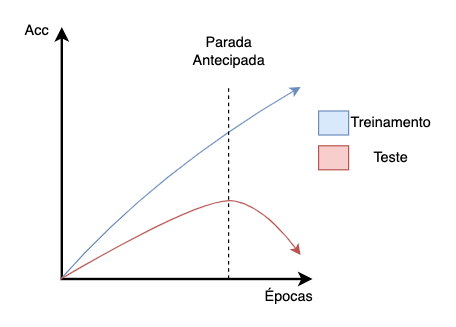
\includegraphics[width=0.6\linewidth]{recursos/imagens/deep/early_stopping.png}
    \label{deep:fig:earlystopping}

    Fonte: do próprio autor.
\end{figure}





\subsubsection{Retro-propagação}
\label{deep:backprop}

Por meio do desenvolvimento de \cite{rumelhart1986learning}, o algoritmo de retro-propagação (ou em inglês, \textit{Backpropagation}) foi capaz de contribuir diretamente no desenvolvimento dos modelos de redes neurais profundas, de modo que esse algoritmo conseguiu realizar o reajuste de pesos em camadas ocultas dos modelos. Com o auxílio de uma função de custo (Seção
\ref{deep:cust}), o erro é calculado na saída da rede $(y)$ e há a propagação do mesmo, iniciando da camada de saída em direção para a camada de entrada. Isso é realizado através do trabalho conjunto do algoritmo \textit{backpropagation} e de um algoritmo de otimização (Seção \ref{deep:optimization}), em que o \textit{backpropagation} realiza um cálculo rápido de gradientes utilizados pelos algoritmos de otimização.

Dessa forma, a explicação dessa Seção se resume em processos em que, dado o erro $E$ que é obtido a partir da saída da rede $(y)$ em relação a um \textit{ground truth} $(g)$, a primeira etapa é realizada com o cálculo da derivada parcial de $E$ em relação a cada neurônio de saída, sendo formada por $\frac{\partial E}{\partial \boldsymbol{y_i}}$ tendo que $i \in \mathbb{K}$ como a representação dos tamanhos de cada saída. Depois, com a aplicação da regra da cadeia de $E$ em relação às entradas $x_j$, é possível obter a seguinte expressão \citep{rumelhart1986learning}:

\begin{equation}
    \label{deep:eq:11}
    \frac{\partial E}{\partial x_j} = \frac{\partial E}{\partial y_j} . \frac{\partial g y_j}{\partial g x_j}.
\end{equation}

A partir da expressão $\frac{\partial E}{\partial x_j}$ é possível visualizar que o erro será afetado na saída ($y$) a medida que a entrada ($x$) for alterada, segundo comentado por \cite{rumelhart1986learning}, que também exemplifica essa função na Equação \ref{deep:eq:12}, ao considerar a entrada como função linear, as conexões do neurônio $i$, assim como os pesos dos neurônios $i$ e $j$:

\begin{equation}
    \label{deep:eq:12}
    \frac{\partial E}{\partial y_j} = \sum_j \frac{\partial E}{\partial x_j . w_{ji}}.
\end{equation}


\subsection{Teste}
\label{deep:test}

A etapa de teste está relacionada com a avaliação do modelo treinado nas condições descritas na Seção \ref{deep:train}, todavia, para a Seção de teste deve-se considerar que o novo conjunto de dados seja desconhecido pela rede neural, ou seja, que não haja intersecção com o conjunto de treinamento, visto que o objetivo do treino está em validar a capacidade de abstração em relação à generalização do modelo.

Entendido isso, habitualmente, é encontrado um conjunto de dados com menos exemplos quando se trata do conjunto de testes \citep{Goodfellow2016}, sendo necessário que ambos os conjuntos de dados, tanto o de teste quanto o de treinamento, possuam uma mesma distribuição dos dados.

O processo de teste pode ser realizado entre as épocas do treinamento, assim, avaliando o desempenho do modelo em um conjunto desconhecido de dados e sendo possível avaliar se a rede está ou não melhorando a capacidade de generalização de acordo com o decorrer das épocas.

Assim, nesta seção são descritos alguns dos elementos utilizados para auxiliar nos teste, como as métricas de avaliação (Seção \ref{deep:metrics}) e o algoritmo \textit{cross validation} (Seção \ref{deep:cross}), além de fenômenos que obstruem o desenvolvimento, como \textit{overfitting} e \textit{underfitting} (Seção \ref{deep:overunder}).


\subsubsection{Métricas de Avaliação}
\label{deep:metrics}

Outro ponto adjutório à avaliação dos modelos, tanto para o conjunto de treinamento quanto para o conjunto de teste são as métricas de avaliação de desempenho, que avaliam o andamento do treinamento do modelo do início ao fim. E referente a classificações, uma métrica que se destaca é a avaliação de acurácia (comumente vista como $Acc$) que pode ser expressa pela Equação \ref{deep:eq:13}:

\begin{equation}
    \label{deep:eq:13}
    Acc = \frac{\text{Quantidade de predições corretas}}{\text{Quantidade de predições realizadas}}.
\end{equation}

A acurácia, como demonstrado na Equação \ref{deep:eq:13}, basicamente se resume entre a razão de acertos pela quantidade total de exemplos no conjunto e é adequada para situações em que se tem o classes balanceadas, mas quando se trata de classes desbalanceadas,o modelo em questão pode apresentar fenômeno de \textit{underfitting} ou \textit{overfitting}, como será explicado na Seção \ref{deep:overunder}, e que podem ser mapeados ao observar o desempenho da acurácia em bases de treino e teste.

Dessa forma, é desejado obter $Acc_{treino} \approx Acc_{teste}$, e com  acurácias altas. Sendo que as situações de \textit{overfitting} possuem a característica de casos em que $Acc_{treino}$ é exacerbadamente mais alto que $Acc_{teste}$. Por outro lado, situações contrárias a essa, tendo $Acc_{treino}$ muito baixos são comuns em casos de \textit{underfitting}.

Já em casos de regressão, o mais comum é utilizarem a métrica MSE, conforme visto na Equação \ref{deep:eq:9}.


\subsubsection{Validação Cruzada}
\label{deep:cross}

Quando se trata na divisão entre os \textit{datasets} de treino e teste, habitualmente é comentado sobre a configuração de 20\% para teste e 80\% para treino, todavia o fato de utilizar um conjunto fixo implica em uma incerteza estatística sobre a média estimada de erro do teste, visto que pode ocorrer um desbalanceamento imprevisto \citep{Goodfellow2016}.

Dessa forma, a validação cruzada (Seção \ref{deep:cross}), do inglês, \textit{cross validation}, trabalha com o principio de divisão entre os \textit{datasets} de treino e teste em subconjuntos que compõem o conjunto de dados original, realizando o cálculos a partir de escolhas de amostras no decorrer das interações. Dentre as técnicas mais conhecidas de \textit{cross validation} para a divisão dos conjuntos de dados, destacam-se os métodos \textit{k-fold} e \textit{leave-one-out}, sendo que preservam o princípio de dividir aleatoriamente o conjunto de dados original em um subconjunto de treinamento e de teste, tendo a premissa de auxiliar a avaliação do algorítimo em relação a sua capacidade de generalização.

Dessa forma, o erro ($\varepsilon$) é computado do teste ($T$) pela média dos erros sobre interações ($\varepsilon_i$) em relação à quantidade de interações($N$), conforme a Equação \ref{deep:eq:15}:

\begin{equation}
    \label{deep:eq:15}
    \varepsilon_T = \frac{1}{N} \sum_{i=1}^{N} \varepsilon_i,
\end{equation}
ou por meio da Equação \ref{deep:eq:16}, quando se refere ao \textit{k-fold cross validation}, ao calcular os testes de erro com base na média dos erros de teste na enésima iteração ($\varepsilon_{Ti}$) em relação a quantidade de \textit{folds} ($k$):

\begin{equation}
    \label{deep:eq:16}
    \varepsilon_T = \frac{1}{k} \sum_{i=1}^{N} \varepsilon_{Ti}.
\end{equation}

\subsubsection{\textit{Overfitting} e \textit{Underfitting}}
\label{deep:overunder}

As situações de \textit{overfitting} e \textit{underfitting} comumente ocorrem quando o modelo está com uma alta variância, em que os dados são \quotes{decorados} no conjunto de treino e não são generalizados quando apresentado a outros dados, como os do conjunto de teste, e, respectivamente, quando apresenta dificuldades de aprendizado, sendo assim caracterizado como um modelo enviesado e não atinge o mínimo de acurácia necessária, a qual normalmente é determinada pelo desenvolvedor.

A partir da representação na Figura \ref{deep:fig:5} é possível exemplificar os fenômenos supracitados, em que na Figura \ref{deep:fig:5}\subref{deep:fig:5.1} se visualiza uma situação característica de \textit{underfitting} ao tentar utilizar um modelo linear para um tipo de problema não linear. Já na imagem \ref{deep:fig:5}\subref{deep:fig:5.2} se encontra uma situação em que há uma função que é utilizada adequadamente para a situação, tendo esta convergido e com uma boa adaptação para demais situações com contextos similares. E, por fim, há a representação de uma situação com \textit{overfitting} na Figura \ref{deep:fig:5}\subref{deep:fig:5.3}, em que o conjunto está decorado e o modelo se ajustou demais ao conjunto de dados - situação que acontece devido ao uso de funções complexas para situações simples.

\begin{figure}[H]
   \caption{Fenômenos de \textit{underfitting} e \textit{overfitting}.}
   \centering
   \label{deep:fig:5}
    \begin{subfigure}[t]{0.45\textwidth}
        \centering
        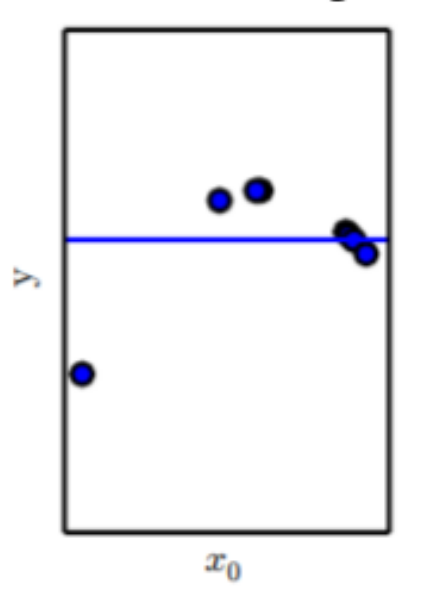
\includegraphics[height=1.5in]{recursos/imagens/deep/under.png}
        \caption{Fenômeno de \textit{underfitting}.}
        \label{deep:fig:5.1}
    \end{subfigure}
    ~ 
    \begin{subfigure}[t]{0.45\textwidth}
        \centering
        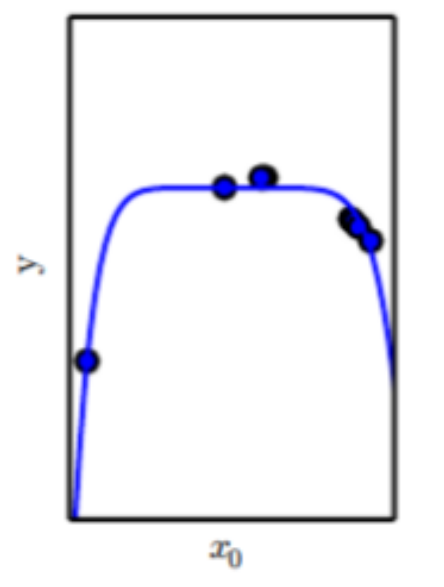
\includegraphics[height=1.5in]{recursos/imagens/deep/apx.png}
        \caption{Representação de função adequada.}
        \label{deep:fig:5.2}
    \end{subfigure}
    ~
    \begin{subfigure}[t]{0.45\textwidth}
        \centering
        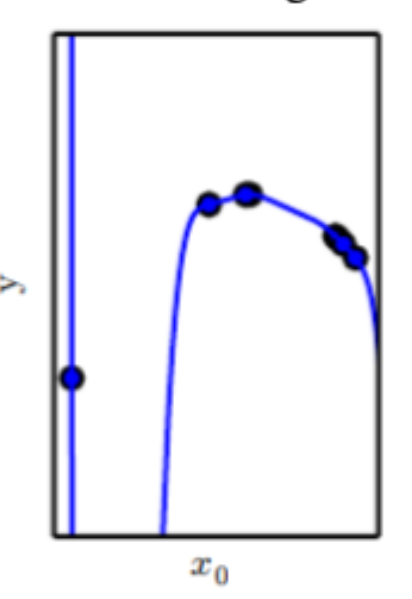
\includegraphics[height=1.5in]{recursos/imagens/deep/over.png}
        \caption{Fenômeno de \textit{overfitting}.}
        \label{deep:fig:5.3}
    \end{subfigure}

    Fonte: retirado e adaptado de \cite{Goodfellow2016}.
\end{figure}

Alerta-se que em situações em que a função de custo de treinamento continua decrescente e a função de custo de teste começa a aumentar, é provavel que o modelo esteja iniciando uma circunstância de \textit{overfitting}, já que casos de \textit{underfitting} ocorrem quando ambas as funções de custo permanecem altas mesmo após muitas épocas.

Sendo assim, \textit{underfitting} e \textit{overfitting}, quando presentes, devem ser corrigidos, embora os ajustes dos métodos à complexidade da situação ainda sejam feitos a partir de tentativa e erro e com o auxílio de gráficos \citep{Goodfellow2016}.

\subsection{Extração de Características}

\subsubsection{\textit{Principal Component Analysis} (PCA)}

\subsection{Considerações Finais do Capítulo}